\subsection{Datos obtenidos}

Se midieron los siguientes valores de resistencias:

\begin{itemize}
        \input{src/1/snippets/resistencias}
\end{itemize}

Los valores medidos de $R_L$, comparados con sus valores nominales, se encuentran en la tabla \ref{tab:1-datos:resistencias-l}.

También se tomaron mediciones de las distintas tensiones presentes en el circuito (tablas \ref{tab:1-datos:tensiones-1} y \ref{tab:1-datos:tensiones-2}) que fueron utilizadas para calcular las corrientes que circulan por cada resistor y cuyos valores se encuentran en la tabla \ref{tab:1-datos:corrientes}.

\begin{table}[H]
    \centering
    \begin{tabular}{@{}rr@{}}
        \toprule
        $R_L$ (nominal, \si{\kilo\ohm}) & $R_L$ (medido, \si{\kilo\ohm})  \\
        \midrule
        \input{src/1/tables/resistencias-l}
    \end{tabular}
    \caption{Valores medidos de $R_L$}
    \label{tab:1-datos:resistencias-l}
\end{table}

\begin{table}[H]
    \centering
    \begin{tabular}{@{}rrrrrr@{}}
        \toprule
        $R_L$ (\si{\kilo\ohm}) & $v_i$ (\si{\volt}) & $v_o$ (\si{\volt}) & 
            $v_+$ (\si{\milli\volt}) & $v_-$ (\si{\milli\volt}) &
            $v_+ - v_-$ (\si{\milli\volt}) \\
        \midrule
        \input{src/1/tables/tensiones-1}
    \end{tabular}
    \caption{Tensiones medidas en el circuito (parte 1)}
    \label{tab:1-datos:tensiones-1}
\end{table}

\begin{table}[H]
    \centering
    \begin{tabular}{@{}rrrrrr@{}}
        \toprule
        $R_L$ (\si{\kilo\ohm}) & $V_{R_1}$ (\si{\volt}) & $V_{R_2}$ (\si{\volt})& $V_{R_3}$ (\si{\milli\volt}) & $V_{R_L}$ (\si{\volt}) \\
        \midrule
        \input{src/1/tables/tensiones-2}
    \end{tabular}
    \caption{Tensiones medidas en el circuito (parte 2)}
    \label{tab:1-datos:tensiones-2}
\end{table}

\begin{table}[H]
    \centering
    \begin{tabular}{@{}rrrrr@{}}
        \toprule
        $R_L$ (\si{\kilo\ohm}) & $I_{R_1}$ (\si{\milli\ampere}) & $I_{R_2}$ (\si{\milli\ampere}) & $I_{R_3}$ (\si{\nano\ampere}) & $I_{R_L}$ (\si{\milli\ampere}) \\
        \midrule
        \input{src/1/tables/corrientes}
    \end{tabular}
    \caption{Corrientes calculadas en el circuito}
    \label{tab:1-datos:corrientes}
\end{table}

La ganancia del operacional puede calcularse experimentalmente como

\begin{equation}
    \label{ec:1-teoria:ganancia-experimental}
    A = \frac{v_o}{v_i}
\end{equation}

\begin{equation}
    \label{ec:1-teoria:err-ganancia-experimental}
    \Delta A = \left| \frac{1}{v_i} \right| \Delta v_o + \left| -\frac{v_o}{{v_i}^2} \right| \Delta v_i
\end{equation}

Los resultados de esta operación se encuentran en la tabla \ref{tab:1-teoria:ganancia-experimental}.


\begin{table}[H]
    \centering
    \begin{tabular}{@{}rr@{}}
        \toprule
        $R_L$ (\si{\kilo\ohm}) & $A$ \\
        \midrule
        \input{src/1/tables/ganancia-experimental}
    \end{tabular}
    \caption{Valores experimentales de ganancia}
    \label{tab:1-teoria:ganancia-experimental}
\end{table}

Teniendo $R_L = \SI{1}{\kilo\ohm}$ se reemplaza la pila de \SI{9}{\volt} por
un generador de funciones configurado para entregar una señal senoidal de
\SI{2}{\volt} de amplitud pico-a-pico y frecuencia $f = \SI{1}{\kilo\hertz}$.
Se conecta también un osciloscopio, cuya pantalla
se muestra en la fig. \ref{fig:1-datos:osciloscopio}. Se observa que la señal
de salida tiene una amplitud muy cercana a la de entrada (\SI{1.02}{\volt} vs.
\SI{1.08}{\volt}), y que se encuentra desfasada en unos \SI{90}{\degree}.

\begin{figure}[H]
    \centering
    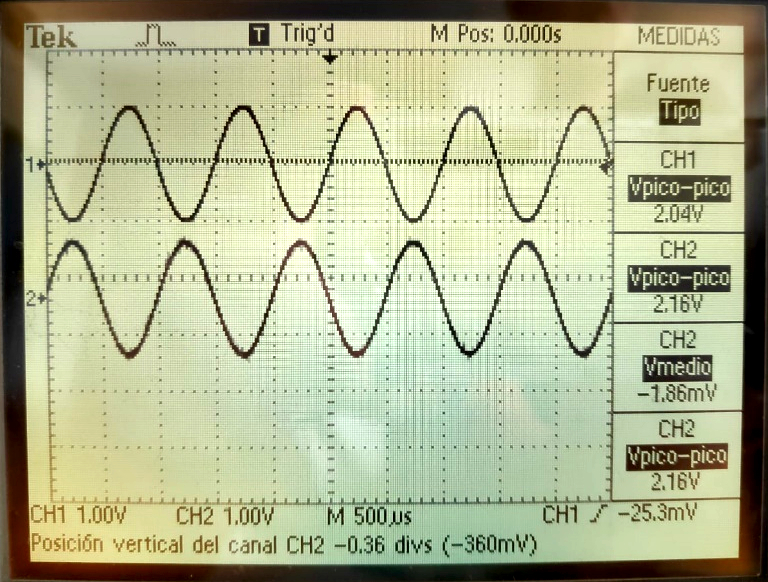
\includegraphics[width=0.8\textwidth]{img/1/osciloscopio-1.jpg}
    \caption{Pantalla del osciloscopio. Se muestran la señal de entrada
        (arriba, canal 1) y la de salida (abajo, canal 2).}
    \label{fig:1-datos:osciloscopio}
\end{figure}
